\documentclass[a4paper,USenglish,english]{lipics-v2018}
%This is a template for producing LIPIcs articles. 
%See lipics-manual.pdf for further information.
%for A4 paper format use option "a4paper", for US-letter use option "letterpaper"
%for british hyphenation rules use option "UKenglish", for american hyphenation rules use option "USenglish"
% for section-numbered lemmas etc., use "numberwithinsect"

\usepackage{microtype}%if unwanted, comment out or use option "draft"

%\graphicspath{{./graphics/}}%helpful if your graphic files are in
%another directory
\graphicspath{{../svg/}}

\bibliographystyle{plainurl}% the recommnded bibstyle

\title{Dummy title}

\titlerunning{Dummy short title}%optional, please use if title is longer than one line

\author{John Q. Public}{Dummy University Computing Laboratory, [Address], Country}{johnqpublic@dummyuni.org}{https://orcid.org/0000-0002-1825-0097}{[funding]}%mandatory, please use full name; only 1 author per \author macro; first two parameters are mandatory, other parameters can be empty.

\author{Joan R. Public}{Department of Informatics, Dummy College, [Address], Country}{joanrpublic@dummycollege.org}{[orcid]}{[funding]}

\authorrunning{J.\,Q. Public and J.\,R. Public}%mandatory. First: Use abbreviated first/middle names. Second (only in severe cases): Use first author plus 'et al.'

\Copyright{John Q. Public and Joan R. Public}%mandatory, please use full first names. LIPIcs license is "CC-BY";  http://creativecommons.org/licenses/by/3.0/

\subjclass{Dummy classification}% mandatory: Please choose ACM 2012 classifications from https://www.acm.org/publications/class-2012 or https://dl.acm.org/ccs/ccs_flat.cfm . E.g., cite as "General and reference $\rightarrow$ General literature" or \ccsdesc[100]{General and reference~General literature}. 

\keywords{Dummy keyword}%mandatory

\category{}%optional, e.g. invited paper

\relatedversion{}%optional, e.g. full version hosted on arXiv, HAL, or other respository/website

\supplement{}%optional, e.g. related research data, source code, ... hosted on a repository like zenodo, figshare, GitHub, ...

\funding{}%optional, to capture a funding statement, which applies to all authors. Please enter author specific funding statements as fifth argument of the \author macro.

\acknowledgements{I want to thank \dots}%optional

%Editor-only macros:: begin (do not touch as author)%%%%%%%%%%%%%%%%%%%%%%%%%%%%%%%%%%
\EventEditors{John Q. Open and Joan R. Access}
\EventNoEds{2}
\EventLongTitle{42nd Conference on Very Important Topics (CVIT 2016)}
\EventShortTitle{CVIT 2016}
\EventAcronym{CVIT}
\EventYear{2016}
\EventDate{December 24--27, 2016}
\EventLocation{Little Whinging, United Kingdom}
\EventLogo{}
\SeriesVolume{42}
\ArticleNo{23}
%\nolinenumbers %uncomment to disable line numbering
%\hideLIPIcs  %uncomment to remove references to LIPIcs series (logo, DOI, ...), e.g. when preparing a pre-final version to be uploaded to arXiv or another public repository
%%%%%%%%%%%%%%%%%%%%%%%%%%%%%%%%%%%%%%%%%%%%%%%%%%%%%%


%%
%% CT
%% Packages not included by LIPICS, but necessary for the work
%%
%% amsthm -- Necessary for \newtheorem
\usepackage{amsthm}
%% subfigure -- Necessary for \subfigure
\usepackage{epsfig}

\begin{document}

\maketitle

%%
%% CT
%% Temporary comment to mark where our modifications begin
%% 

%% \addcite -- Adds a bit of bright text reminding the author a
%% citation is needed.
%% Usage: \addcite{}
\newcommand{\addcite}{({\color{red}\emph{citation}})}

%% \revise -- Colors a block of text indicating it needs to be
%% rewritten
%% Usage: \revise{ TEXT }
\newcommand*{\revise}{\textcolor{red}}


% Task Set - \tasks
\newcommand{\tasks}{\ensuremath{\tau}}
% Individual Task - \task{n}
\newcommand{\task}[1]{\ensuremath{\tau_{#1}}}
% Minimum inter-arrival time - \period{n}
\newcommand{\period}[1]{\ensuremath{T_{#1}}}
% Relative deadline - \deadline{n}
\newcommand{\deadline}[1]{\ensuremath{d_{#1}}}
% Absolute deadline - \Deadline{n}
\newcommand{\Deadline}[1]{\ensuremath{D_{#1}}}
% DAG set - \dagset
\newcommand{\dagset}{\ensuremath{\mathbb{G}}}
% Individual DAG
%	\Dag{i}	->	G_i
%	\Dag{}	->	G
\newcommand{\Dag}[1]{\ifx &#1& \ensuremath{G} \else \ensuremath{G_{#1}} \fi}
% set of nodes in a DAG
%	\nodeset{i}	->	V_i
%	\nodeset{}		->	V
\newcommand{\nodeset}[1]{\ifx &#1& \ensuremath{V} \else \ensuremath{V_{#1}} \fi}

% set of edges in a DAG
%	\edgeset{i}	->	E_i
%	\edgeset{}		->	E
\newcommand{\edgeset}[1]{\ifx &#1& \ensuremath{E} \else \ensuremath{E_{#1}} \fi}
% node
%	\node{0}	->	u
%	\node{1}	->	v
%	\node{2}	->	w
%	\node{3}	->	t
\newcommand{\node}[1]{\ifx 0#1 \ensuremath{u} \fi \ifx 1#1 \ensuremath{v} \fi \ifx 2#1 \ensuremath{w} \fi \ifx 3#1 \ensuremath{t} \fi}
%edge - \edge
\newcommand{\edge}{\ensuremath{e}}

%parent - \parent
\newcommand{\parent}[1]{\ensuremath{parent(#1)}}
%child - \child
\newcommand{\child}[1]{\ensuremath{child(#1)}}
%predecessors - \pred
\newcommand{\pred}[1]{\ensuremath{pred(#1)}}
%successors - \succ
\newcommand{\successor}[1]{\ensuremath{succ(#1)}}

%critical path
%	\criticalpath{i}	->	\lambda_i
%	\criticalpath{}	->	\lambda 
\newcommand{\criticalpath}[1]{\ifx &#1& \ensuremath{\lambda} \else \ensuremath{\lambda_{#1}} \fi}
%critical path length 
%	\criticalpathlen{i}	->	L_i
%	\ciriticalpathlen{}	->	L
\newcommand{\criticalpathlen}[1]{\ifx &#1& \ensuremath{L} \else \ensuremath{L_{#1}} \fi}


%workload of a DAG task
% 	\workload{} -> C
%	\workload{i} -> C_i
\newcommand{\workload}[1]{\ifx &#1& \ensuremath{C} \else \ensuremath{C_{#1}} \fi}
% number of cores assigned to a task - \noofcores{i}
\newcommand{\noofcores}[1]{\ensuremath{m_{#1}}}
% total number of cores available  - \totalcores
\newcommand{\totalcores}{\ensuremath{m}}

%WCET - \wcet{n}
\newcommand{\wcet}[1]{\ensuremath{\ifx &#1& \ensuremath{c} \else \ensuremath{c_{#1}} \fi }}
% WCET - \newwcet{n}{m} or \newwcet{}{m}
%    n - task number
%    m - number of threads
\newcommand{\newwcet}[2]{\ensuremath{\ifx &#1& \ensuremath{c{(#2)}} \else \ensuremath{c_{#1}{(#2)}} \fi }}

%block reload time (BRT) - \brt
\newcommand{\brt}{\ensuremath{\mathbb{B}}}
%code segment - \cs{\node0}
\newcommand{\cs}[1]{\ensuremath{\alpha_{#1}}}
%number of threads executing one node - \noofthreads{\node0}
\newcommand{\noofthreads}[1]{\ensuremath{\eta_{#1}}}

% SLACK - \slack{${D_i}$}
\newcommand{\slack}[1]{\text{\sc{slack}(#1)}}
% DBF - \dbf{\tau_i}{\Deadline{k}}
\newcommand{\dbf}[2]{\text{\sc{dbf}(#1,#2)}}
% Hyper Period - \hp
\newcommand{\hp}{\ensuremath{P}}

\section{System Model}

\subsection{Task Model}
We consider a task set $\tau$ of ${n}$ sporadic parallel real time tasks,
$\tau = \{\tau_1,\tau_2, ..., \tau_n\}$. A task $\tau_i$ in the task
system generates a potentially infinite number of jobs, each arriving
no less than $T_i$ time units after the previous job and has a constrained
deadline $D_i$ where $D_i \leq T_i$.  Each task $\tau_i \in \tau$ is
considered as a parallel task and is represented as a directed acyclic
graph (DAG) ${G_i}$, the set of DAGs is given as ${G = \{G_1, G_2,
  ..., G_n\}}$. An example DAG is shown in Fig.~\ref{fig:dag}.

\begin{figure}[!h]
  \centering
  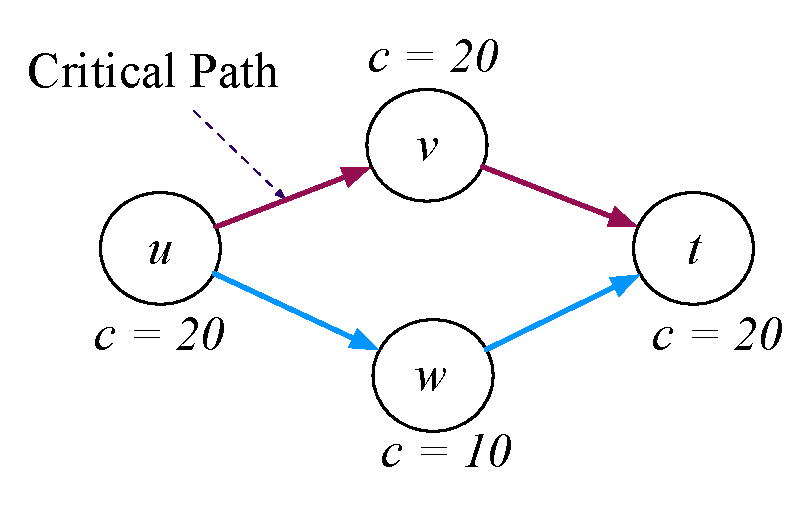
\includegraphics[width=0.4\columnwidth]{dag}
  \caption{An Example of a Parallel Real-time Task}
  \label{fig:dag}
\end{figure}

\revise{A node $v_i^j \in V_i$ is expressed as a double <$cs_i^j$, $c_i^j$>, where $cs_i^j$ denotes the code segment executed by a thread and $c_i^j$ denotes the worst-case execution time of the thread execution.}
Each node ${v \in V_i}$ of a DAG ${G_i = (V_i, E_i)}$ represents the
execution of a thread and an ${e \in E_i}$ edge represents a
dependency between two nodes. A dependency between two nodes indicates
that a node is ready to execute only upon the completion of all its
predecessor nodes. We consider a source as a node with no incoming
arcs and a sink as node with no outgoing arcs. For the sake of
simplicity, we assume a task has only one source and sink node. In
practice, this not hard to achieve as a source and sink can be added
to the task with $0$ execution and not change the task dependencies.

%Nodes of a task have an associated worst-case execution time. 
\revise{For a node $v_i^j$, we define $parent(v_i^j)$ and $child(v_i^j)$ as a set of parent nodes of $v_i^j$ and a set of child nodes of $v_i^j$, respectively. we define $pre(v_i^j)$ and $succ(v_i^j)$ as a set of all predecessors of $v_i^j$ and a set of all successors of $v_i^j$, respectively.}
For any given task, we define a \textit{critical path} $\lambda_i$ of a 
task $\tau_i$ as the longest execution time path that starts from
source and ends at the sink. \textit{Critical path length} ($L_i$) is
defined as the sum of execution times of all nodes along the critical
path $\lambda_i$ of task $\tau_i$.  Workload $C_i$ of
a task $\tau_i$ is defined as the sum of worst-case execution time of
all nodes in the DAG task. 


\subsection{Federated Scheduler}
For a task set $\tau$ , the federated scheduling algorithm works as
follows. We first divide the task sets into two disjoint sets
$\tau_{high}$  and $\tau_{low}$. $\tau_{high}$ contains all tasks with
high utilization (i.e. $u_i > 1$) and $\tau_{low}$ contains all
remaining low utilization tasks. Each task in $\tau_{high}$ is
assigned $m_i$ dedicated cores (no other task is executed on these
cores), where: \begin{equation}\label{eq:m} m_i = \left\lceil \frac{C_i - L_i}{D_i - L_i}
\right\rceil \end{equation}

We use $m_{high} = \sum_{\tau_i \in \tau_{high}} m_i$ to denote the total
number of cores assigned to high-utilization tasks. We assign
the remaining cores to all low-utilization tasks $\tau_{low}$, denoted
as ${m_{low} = m - m_{high}}$. The federated scheduling algorithm admits
the task set ${\tau}$, if $m_{low}$ is non-negative and all tasks in
$\tau_{low}$ are schedulable sequentially.  

After a valid core allocation, runtime scheduling proceeds as
follows. Any greedy (work-conserving) parallel scheduler can be used
to schedule a high-utilization task $\tau_i \in \tau_{high}$ on its
assigned $m_i$ cores. Informally, a greedy scheduler is one that never
keeps a core idle if some node is ready to execute. 

All low-utilization tasks are treated and executed as though they are
sequential tasks and any multiprocessor scheduling algorithm (such as
partitioned EDF, or various rate-monotonic schedulers) can be used to
schedule all the low-utilization tasks on the allocated $m_{low}$
cores. We can safely treat low-utilization tasks as sequential tasks
since $C_i \le D_i$ and parallel execution is not required to meet their
deadlines. 

\subsection{Processing Model}

In this work, for each core, we assume a dedicated direct mapped
instruction cache. We assume a time-compositional architecture\addcite,
where memory and execution demand are separable. Copying a block of 
main memory to cache memory requires ${\mathbb{B}}$ cycles, commonly
referred to as the the block reload time (BRT). If multiple cores share
the same processing platform their cache contents do not interfere with
one another. The impact of a shared cache between cores is not considered.


\section{Proposed Changes to the Directed Acyclic Graph Model of Parallel Systems}

For a DAG ${G = (V, E)}$ representing a parallel task, each node ${v_i \in V}$ represents
the release, execution, and termination of a single thread within one task 
\addcite. In the existing model, the only relationship between thread releases and the executable object they execute is the worst-case execution time of the node. Two nodes ${v_i, v_j \in V}$ may represent two threads executing the same object (possibly on different processors).

\begin{figure}
  \centering
  \begin{subfigure}[b]{0.4\textwidth}{
      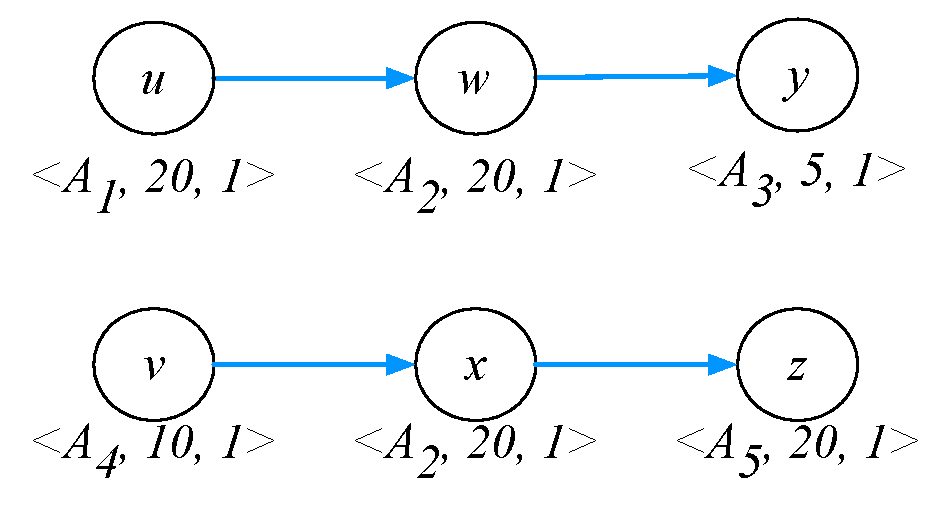
\includegraphics[width=\textwidth]{beforeCollapse}
      \caption{Before Collapse}
      \label{fig:before-collapse}
    }
  \end{subfigure} \quad
  \begin{subfigure}[b]{0.4\textwidth}{
      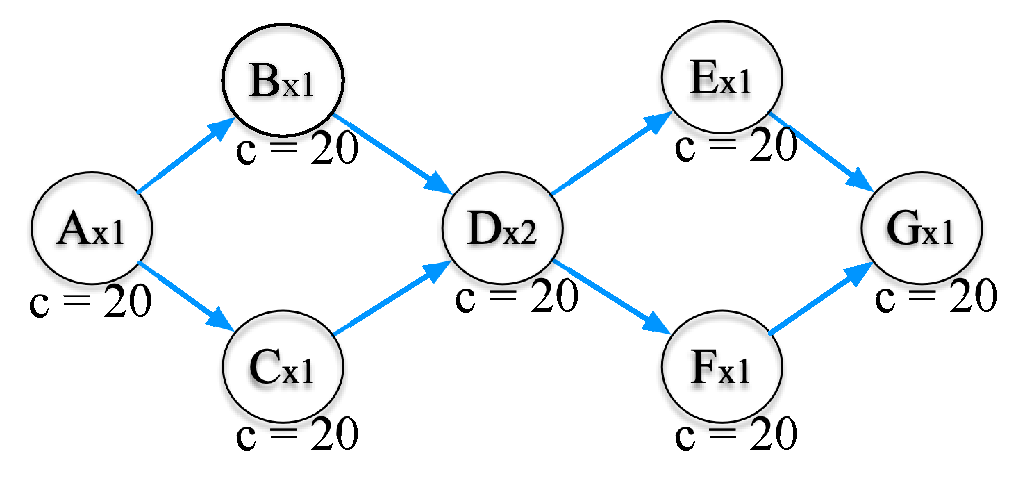
\includegraphics[width=\textwidth]{afterCollapse}
      \caption{After Collapse}
      \label{fig:after-collapse}
    }
  \end{subfigure}
  \caption{DAG Node Change from Thread to Code Segment}
  \label{fig:dag-change}
\end{figure}

To take advantage of instruction cache reuse, we propose a simple modification to the DAG
model. Where possible, distinct nodes that represent the execution of
the same object are collapsed into a single node. To accommodate collapse,
nodes are identified by their executable object, and a new attribute is added to every node
indicating the number of threads which will be executed over the object.

\revise{Given the new model to represent a node, two nodes $v_i^j$, $v_i^k$ with the same code segments (i.e., $cs_i^j = cs_i^k$ and $c_i^j = c_i^k$) are collapsed into one node $v_i^h$, where $v_i^h = <cs_i^j, c_i^j, \max{\eta_i^j, \eta_i^k}+1>$.  To ensure dependencies of the DAG are not violated, we replace the edges that start from $v_i^j$ and $v_i^k$  to start from $v_i^h$, i.e., the child nodes of $v_i^h$ are given as a union of the child nodes of $v_i^j$ and $v_i^k$, $child(v_i^h) = child(v_i^j) \cup child(v_i^k)$. Similarly, parent nodes of $v_i^h$ are given as a union of the parent nodes of $v_i^j$ and $v_i^k$, i.e., $parent(v_i^h) = parent(v_i^j) \cup parent(v_i^k)$.}

Figure~\ref{fig:dag-change} illustrates the proposed change. Nodes in
Figure~\ref{fig:before-collapse} are labeled with the code segment
they are associated with. Two nodes of ${B}$ are collapsed in
Figure~\ref{fig:after-collapse}, where each node is attributed with
the number of threads executed over the code segment.

A goal of this work is to bring the inter-thread cache benefit \addcite to parallel DAG tasks. 

%% ct - commented out because splitting a code segment into multiple code segments may introduce loops in the DAG. 
%%		For example, if a loop is too big and cannot fit into a cache block then we it will be split across multiple segments which will introduce a DAG.
%%
%%A goal of this work is to bring the inter-thread cache benefit \addcite to parallel DAG tasks. As a first-step, two requirements are placed on nodes of the graph.
%%\begin{description}
%%\item[R1] All executable objects must fit entirely within the cache.
%%\item[R2] No two instructions of an executable object may evict one another.
%%\end{description}
%%
%%Requirements R1 and R2 may be met for any executable object by repeatedly dividing
%%the object source that result in objects larger than the cache into separate code segments, carefully recompiling those code segments to maximize cache use, and replacing the original node with a serial set of nodes.
%%\\
%%\\
%%\emph{ct-3 A figure is needed to illustrate the transformation from one over-sized node, to multiple correctly sized nodes}
%%\\

In the established model \addcite, each node ${v_i^j \in V_i}$ is characterized
with a single worst case execution time for a single thread. We
propose that each node's WCET is characterized by a function
${c_i^j(\eta_i^j)}$ where ${\eta_i^j}$ is the number of threads that will execute the
node ${v_i^j}$ on the same core serially (one after another) with no
other thread executing a different object on the core in between executions.

%%Given a timing-compositional architecture with the restrictions \textbf{R1} and \textbf{R2},
Given a timing-compositional architecture
${c_i(n)}$ can be expressed for any node in terms of the memory demand of all instructions
of ${v_j \in V_i}$ into the cache ${\gamma_j}$ and the worst-case execution demand
to execute the node assuming all instructions of ${v_j}$ have
been cached ${\iota_j}$. Equation~\ref{eq:c_i} is an expression for
${c_i(n)}$. 
 
\begin{equation}
  \label{eq:c_i}
  c_i(n) = \begin{cases}
    0, & n \le 0 \\
    \gamma_j + \iota_j \cdot n, & n > 0
  \end{cases}
\end{equation}

For a node ${v_i \in V_j}$, the upper bound of memory demand of the node is denoted ${\gamma_i}$. It is the number of cycles required to load all blocks of the node. The complete set of blocks of the node are equivalent to the evicting cache blocks (ECBs)\addcite [Tan \& Mooney] of the object. Thus, the memory demand is the product of the BRT and count of ECBs of the node ${\textsc{ecb}_i}$ found in Equation~\ref{eq:mem-demand}.

\begin{equation}{\label{eq:mem-demand}}
    \gamma_i = \mathbb{B} \cdot \textsc{ecb}_i
\end{equation}

The execution demand ${\iota_i}$ for a node ${v_i^j \in V_i}$ is the worst case execution time of a single thread given all instructions are present in the cache. Any suitable WCET calculation method {\addcite} may be used to calculate the value.

%%\section{Problem Formulation}

\section{Proposed Method - For High Utilization Tasks}
\revise{We define candidates for collapse as a pair of nodes that share the same cache block, and other conditions. Identifying potential candidates for collapse is discussed in the following/previous section. For this section, we assume that the potential candidates are at the same depth from the start node and they are not dependent on each other. } 

In a federated scheduler, a high utilization task $T_i$ is allocated $m_i$ dedicated cores, given by Equation (\ref{eq:m}), where no other tasks can execute. In this environment, collapsing two nodes in the DAG of high utilization task $T_i$ is beneficial to the federated scheduler if the collapse decreases the required number of cores. Formally, consider the number of cores dedicated to a task ${T_i}$ before any two nodes are collapsed as ${m_i}$ as calculated by Equation~\ref{eq:m}. The number of cores dedicated to ${T_i}$ after collapse are denoted ${\hat{m}_i}$.

\textbf{Beneficial Collapse}: Collapsing two nodes of a task ${T_i}$ is \emph{beneficial} if ${\hat{m}_i \le m_i}$.

\revise{We need more supportive definitions before the proof, \\ 
  1 inter-thread cache benefit for two collapsed nodes ${v_j}$ and ${v_k}$ for the same executable object \\
  2 max extension of paths by ${\iota_j}$ for two collapsed nodes ${v_j}$ and ${v_k}$. \\
  3 "resulting path" -- the single path that results from ${v_j}$ and ${v_k}$ being collapsed from separate paths
  }

In Theorem~\ref{thrm:conditional-collapse}, we derive a sufficient condition to determine if collapsing two nodes is beneficial. The proof is divided into four sections. Each is related to the impact of collapse upon the longest path through the DAG of ${T_i}$.

%\newtheorem{theorem}{Theorem}
\begin{theorem}[Conditional Collapse]\label{thrm:conditional-collapse} For a DAG task ${\tau_i}$, collapsing two \textbf{candidate} nodes ${v_j, v_k \in V_i}$ (which refer to the same executable object) is \textbf{beneficial} if:

    \begin{equation}\label{eq:cond}
        1 + \frac{\gamma_j}{\iota_j} > \frac{C_i  - L_i }{D_i - L_i}
    \end{equation}
\end{theorem}
\begin{proof}
A direct proof supports the theorem, it is divided into four cases 1.) collapsing two nodes off the critical path where the critical path length is not affected 2.) collapsing two nodes with exactly one lies on the critical path 3.) collapsing two nodes where both lie on the critical path 4.) collapsing two nodes off the critical path, which creates a new critical path length.

\emph{Case 1.} Collapsing two nodes off the critical path with no impact to the critical path length. Since ${v_j}$ and ${v_k}$ refer to the same executable object ${\iota_j = \iota_k}$ and ${\gamma_j = \gamma_k}$. Collapsing ${v_j}$ and ${v_k}$ in the graph serializes the execution of threads on the same processor. This decreases the execution time ${v_k}$ (or ${v_j}$) due to the inter-thread cache benefit; which is quantified as ${2 \cdot \iota_j + \gamma_j}$. This increases the path(s) of ${v_j}$ and ${v_k}$ by at most ${\iota_j}$. 
\end{proof}
%\end{theorem}
%\blacksquare

Collapsing two nodes of DAG tasks always results in a decrease in the worst-case execution time of the task by $\mathbb{B}$. Nevertheless, collapsing two nodes of DAG tasks may increase the critical path by $\mathbb{I}$, may increase the critical path by a value less than $\mathbb{I}$ but greater than $0$, or may not change the critical path length value. For example, Fig.~\ref{fig:c1}, Fig~\ref{fig:c2}, and Fig.~\ref{fig:c3} show the three cases, i.e., case 1 when there is no change in critical path length, case 2 when the critical path length increases by $\mathbb{I}$, and case 3 when the critical path length increases by a values greater than $0$ but less than $\mathbb{I}$.

\begin{figure}
  \centering
  \begin{subfigure}[b]{0.4\textwidth}{
      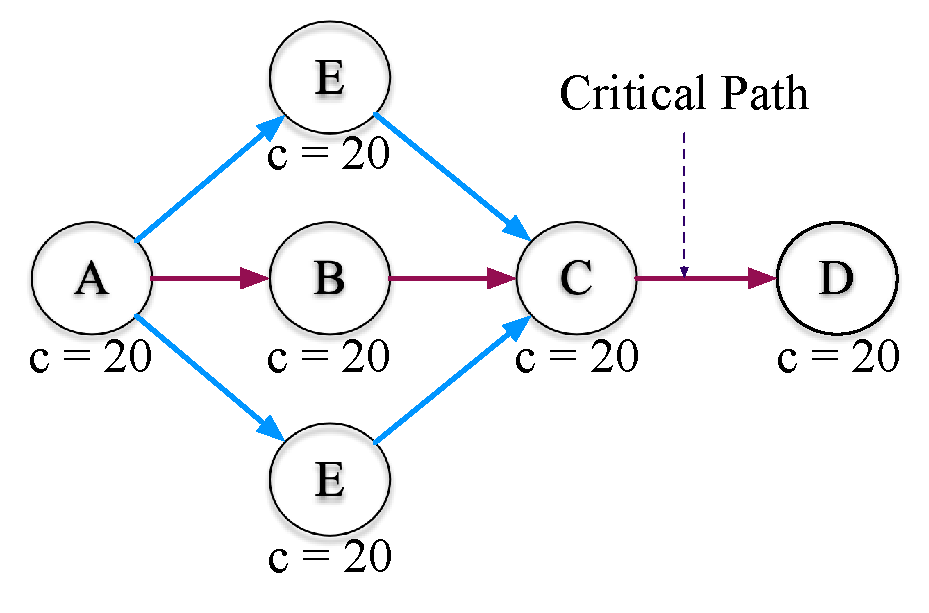
\includegraphics[width=\textwidth]{c1before}
      \caption{Before Collapse}
      \label{fig:c1before}
    }
  \end{subfigure}~
  \begin{subfigure}[b]{0.4\textwidth}{
      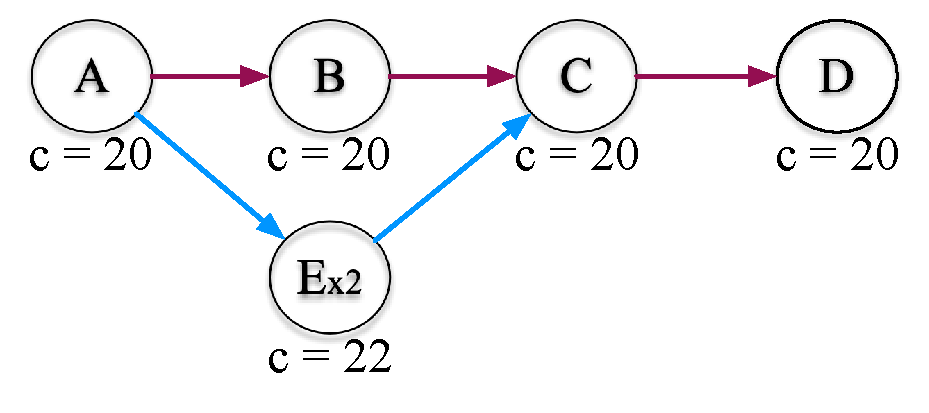
\includegraphics[width=\textwidth]{c1after}
      \caption{After Collapse}
      \label{fig:c1after}
    }
  \end{subfigure}
  \caption{Case 1:  No change in the critical path length}
  \label{fig:c1}
\end{figure}

\begin{figure}
  \centering
  \begin{subfigure}[b]{0.4\textwidth}{
      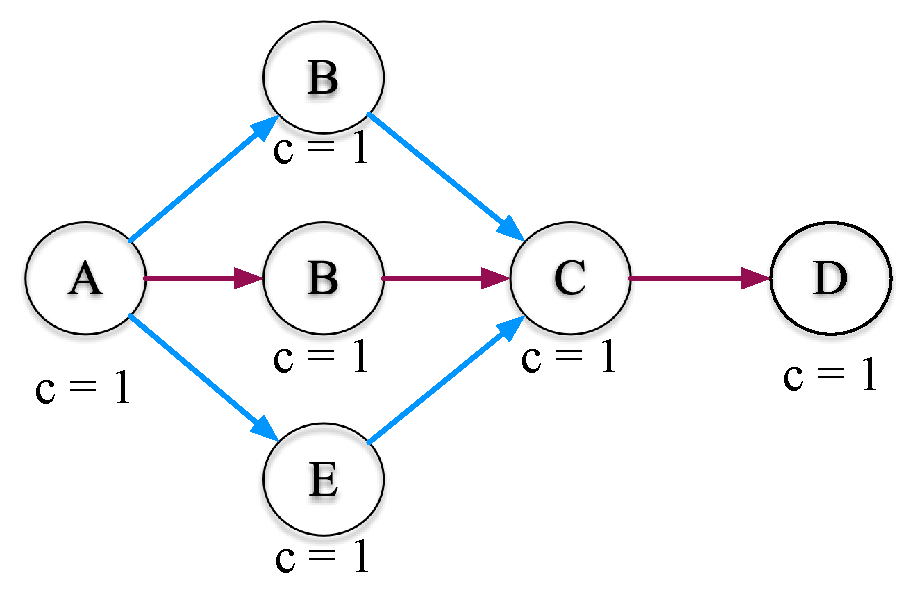
\includegraphics[width=\textwidth]{c2before}
      \caption{Before Collapse}
      \label{fig:c2before}
    }
  \end{subfigure}~
  \begin{subfigure}[b]{0.4\textwidth}{
      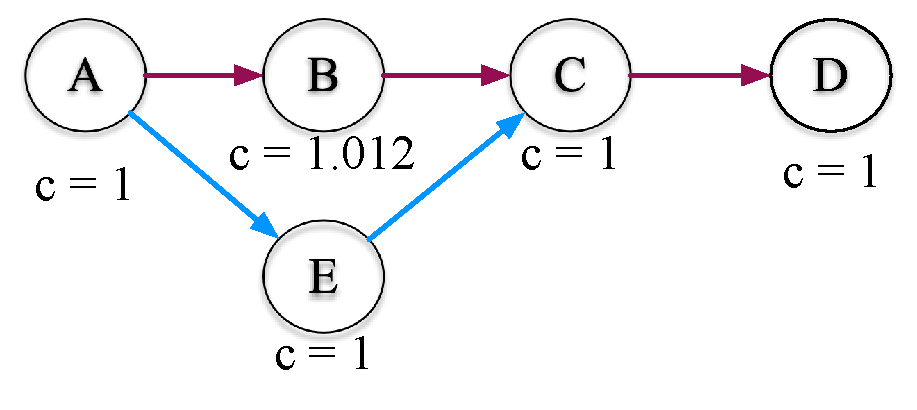
\includegraphics[width=\textwidth]{c2after}
      \caption{After Collapse}
      \label{fig:c2after}
    }
  \end{subfigure}
  \caption{Case 2:  Critical path length increases by $\mathbb{I}$}
  \label{fig:c2}
\end{figure}

\begin{figure}
  \centering
  \begin{subfigure}[b]{0.4\textwidth}{
      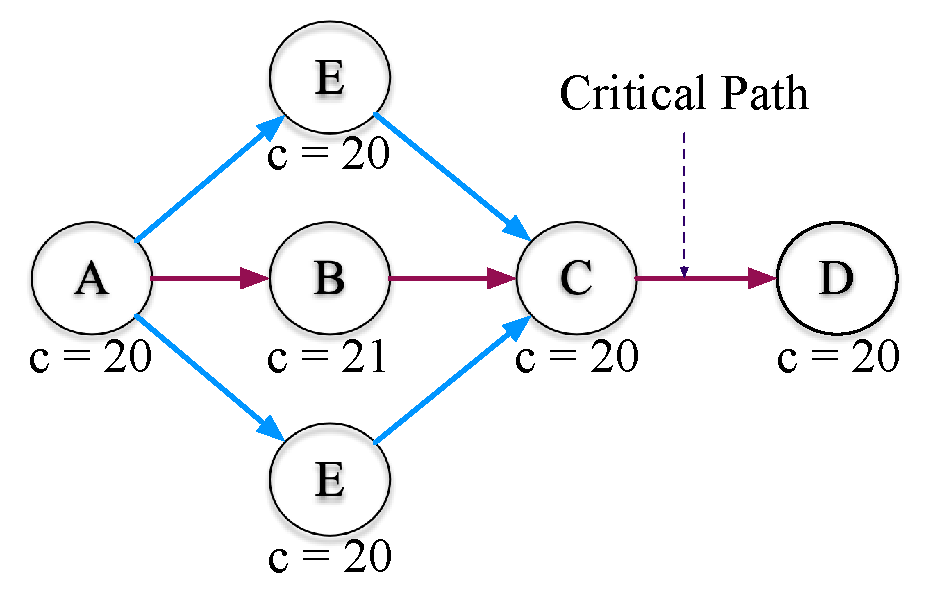
\includegraphics[width=\textwidth]{c3before}
      \caption{Before Collapse}
      \label{fig:c2before}
    }
  \end{subfigure}~
  \begin{subfigure}[b]{0.4\textwidth}{
      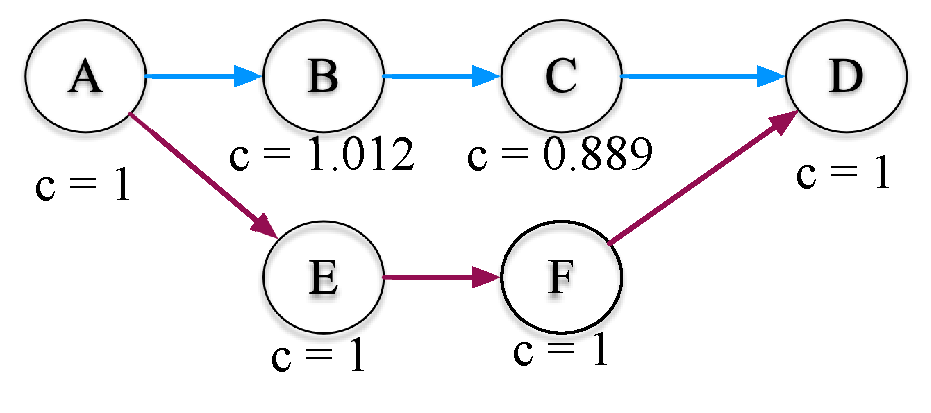
\includegraphics[width=\textwidth]{c3after}
      \caption{After Collapse}
      \label{fig:c2after}
    }
  \end{subfigure}
  \caption{Case 3:  Critical path length increases by a value less than $\mathbb{I}$}
  \label{fig:c3}
\end{figure}

In case 1, there is no change in the critical path length but the worst case execution decreases by $\mathbb{B}$,thus the required number of cores after collapse, given by $\frac{C_i - \mathbb{B} - L_i}{D_i - L_i}$, is less than the required number of cores before collapse, given by $\frac{C_i - L_i}{D_i - L_i}$  (since $\frac{C_i - \mathbb{B} - L_i}{D_i - L_i} < \frac{C_i - L_i}{D_i - L_i}$). Therefore, any two nodes that fall under case 1 can be considered for collapse. 

In case 2, the task $T_i$ saves $\mathbb{B}$ units of worst-case execution time however it increases the critical path length by $\mathbb{I}$. Similarly, in case 3, the task $T_i$ saves $\mathbb{B}$ units of worst-case execution time however it increases the critical path length by at most $\mathbb{I}$. To derive a sufficient condition, we consider the upper bound on the increase in critical path length, i.e., $\mathbb{I}$ as the increase in critical path length. Thus, under case 2 and 3, a task receives a saving of $\mathbb{B}$ in worst-case execution time but spends $\mathbb{I}$ on the critical path. In case 2 and 3, collapsing two nodes can decrease the number of cores if Equation (\ref{eq:cond}) holds.

\begin{equation} \label{eq:cond} 1 + \frac{\mathbb{B}}{\mathbb{I}} > \frac{C_i  - L_i }{D_i - L_i} \end{equation}

To prove this, let us assume the Equation (\ref{eq:inequality}) is true.
\begin{equation} \label{eq:inequality} \frac{C_i - \mathbb{B} - (L_i + \mathbb{I})}{D - (L_i + \mathbb{I})}  < \frac{C_i  - L_i }{D_i - L_i} \end{equation}
Then by algebraic simplification, the following inequality is also true.
$$ - ( \mathbb{B} + \mathbb{I}) (D_i - L_i)  < -\mathbb{I}(C_i  - L_i )$$
Further simplification shows that the following inequality is also true.
$$ 1 + \frac{\mathbb{B}}{\mathbb{I}} > \frac{C_i  - L_i }{D_i - L_i}$$
Since the obtain result is obtained from algebraic simplification of Equation (ref{eq:inequality}), we can conclude that if Equation (\ref{eq:cond}) is true then Equation (\ref{eq:inequality}) is also true.


\clearpage

%%
%% CT
%% Leaving the remaining instructions within the main document until
%% we have incorporated all of them.
%%
they have been incorporated into our work.
\begin{abstract}
Lorem ipsum dolor sit amet, consectetur adipiscing elit. Praesent convallis orci arcu, eu mollis dolor. Aliquam eleifend suscipit lacinia. Maecenas quam mi, porta ut lacinia sed, convallis ac dui. Lorem ipsum dolor sit amet, consectetur adipiscing elit. Suspendisse potenti. 
 \end{abstract}

\section{Typesetting instructions -- please read carefully}
Please comply with the following instructions when preparing your article for a LIPIcs proceedings volume. 
\begin{itemize}
\item Use pdflatex and an up-to-date LaTeX system.
\item Use further LaTeX packages only if required. Avoid usage of packages like \verb+enumitem+, \verb+paralist+, \verb+cleverref+. Keep it simple, i.e. use as few additional packages as possible.
\item  The \texttt{enumerate} package is preloaded, so you can use
 \verb+\begin{enumerate}[(a)]+ or the like.
\item Add custom made macros carefully and only those which are needed in the article (i.e., do not simply add your convolute of macros collected over the years).
\item Do not use a different main font. For example, the usage of the \verb+times+-package is forbidden.
\item Provide full author names (especially with regard to the first name) in the \verb+\author+ macro and in the \verb+\Copyright+ macro.
\item Provide only one author per \verb+\author+ macro, even if two or more authors have the same affiliation.
\item Fill out the \verb+\subjclass+ and \verb+\keywords+ macros. For the \verb+\subjclass+, please refer to the ACM classification at \url{https://www.acm.org/publications/class-2012}.
\item If you refer to a longer version of the paper (``full version''), please make sure to provide a persistent URL, e.g., at arXiv. Please  mention this full version using the \verb+\relatedversion+ macro.
\item Take care of suitable linebreaks and pagebreaks. No overfull \verb+\hboxes+ should occur in the warnings log.
\item Provide suitable graphics of at least 300dpi (preferrably in pdf format).
\item Use the provided sectioning macros: \verb+\section+, \verb+\subsection+, \verb+\subsection*+, \verb+\paragraph+, \verb+\subparagraph*+, ... ``Self-made'' sectioning commands (for example, \verb+\noindent{\bf My+ \verb+subparagraph.}+ will be removed and replaced by standard LIPIcs style sectioning commands.
\item Do not alter the spacing of the  \verb+lipics-v2018.cls+ style file. Such modifications will be removed.
\item Do not use conditional structures to include/exclude content. Instead, please provide only the content that should be published -- in one file -- and nothing else.
\item Remove all comments, especially avoid commenting large text blocks and using \verb+\iffalse+ $\ldots$ \verb+\fi+ constructions.
\item Keep the standard style (\verb+plainurl+) for the bibliography as provided by the\linebreak \verb+lipics-v2018.cls+ style file.
\item Use BibTex and provide exactly one BibTex file for your article. Please make sure that there are no errors and warnings with the referenced BibTex entries.
\item Use a spellchecker to get rid of typos.
\item A manual for the LIPIcs style is available at \url{http://drops.dagstuhl.de/styles/lipics-v2018/lipics-v2018-authors/lipics-v2018-manual.pdf}.
\end{itemize}


\section{Lorem ipsum dolor sit amet}

Lorem ipsum dolor sit amet, consectetur adipiscing elit \cite{DBLP:journals/cacm/Knuth74}. Praesent convallis orci arcu, eu mollis dolor. Aliquam eleifend suscipit lacinia. Maecenas quam mi, porta ut lacinia sed, convallis ac dui. Lorem ipsum dolor sit amet, consectetur adipiscing elit. Suspendisse potenti. Donec eget odio et magna ullamcorper vehicula ut vitae libero. Maecenas lectus nulla, auctor nec varius ac, ultricies et turpis. Pellentesque id ante erat. In hac habitasse platea dictumst. Curabitur a scelerisque odio. Pellentesque elit risus, posuere quis elementum at, pellentesque ut diam. Quisque aliquam libero id mi imperdiet quis convallis turpis eleifend. 

\begin{lemma}[Lorem ipsum]
\label{lemma:lorem}
Vestibulum sodales dolor et dui cursus iaculis. Nullam ullamcorper purus vel turpis lobortis eu tempus lorem semper. Proin facilisis gravida rutrum. Etiam sed sollicitudin lorem. Proin pellentesque risus at elit hendrerit pharetra. Integer at turpis varius libero rhoncus fermentum vitae vitae metus.
\end{lemma}

\begin{proof}
Cras purus lorem, pulvinar et fermentum sagittis, suscipit quis magna.
\end{proof}

\begin{theorem}[Curabitur pulvinar, \cite{DBLP:books/mk/GrayR93}]
\label{theorem:curabitur}
Nam liber tempor cum soluta nobis eleifend option congue nihil imperdiet doming id quod mazim placerat facer possim assum. Lorem ipsum dolor sit amet, consectetuer adipiscing elit, sed diam nonummy nibh euismod tincidunt ut laoreet dolore magna aliquam erat volutpat.
\end{theorem}

\subsection{Curabitur dictum felis id sapien}

Curabitur dictum felis id sapien mollis ut venenatis tortor feugiat. Curabitur sed velit diam. Integer aliquam, nunc ac egestas lacinia, nibh est vehicula nibh, ac auctor velit tellus non arcu. Vestibulum lacinia ipsum vitae nisi ultrices eget gravida turpis laoreet. Duis rutrum dapibus ornare. Nulla vehicula vulputate iaculis. Proin a consequat neque. Donec ut rutrum urna. Morbi scelerisque turpis sed elit sagittis eu scelerisque quam condimentum. Pellentesque habitant morbi tristique senectus et netus et malesuada fames ac turpis egestas. Aenean nec faucibus leo. Cras ut nisl odio, non tincidunt lorem. Integer purus ligula, venenatis et convallis lacinia, scelerisque at erat. Fusce risus libero, convallis at fermentum in, dignissim sed sem. Ut dapibus orci vitae nisl viverra nec adipiscing tortor condimentum \cite{DBLP:journals/cacm/Dijkstra68a}. Donec non suscipit lorem. Nam sit amet enim vitae nisl accumsan pretium. 

\begin{lstlisting}[caption={Useless code},label=list:8-6,captionpos=t,float,abovecaptionskip=-\medskipamount]
for i:=maxint to 0 do 
begin 
    j:=square(root(i));
end;
\end{lstlisting}

\subsection{Proin ac fermentum augue}

Proin ac fermentum augue. Nullam bibendum enim sollicitudin tellus egestas lacinia euismod orci mollis. Nulla facilisi. Vivamus volutpat venenatis sapien, vitae feugiat arcu fringilla ac. Mauris sapien tortor, sagittis eget auctor at, vulputate pharetra magna. Sed congue, dui nec vulputate convallis, sem nunc adipiscing dui, vel venenatis mauris sem in dui. Praesent a pretium quam. Mauris non mauris sit amet eros rutrum aliquam id ut sapien. Nulla aliquet fringilla sagittis. Pellentesque eu metus posuere nunc tincidunt dignissim in tempor dolor. Nulla cursus aliquet enim. Cras sapien risus, accumsan eu cursus ut, commodo vel velit. Praesent aliquet consectetur ligula, vitae iaculis ligula interdum vel. Integer faucibus faucibus felis. 

\begin{itemize}
\item Ut vitae diam augue. 
\item Integer lacus ante, pellentesque sed sollicitudin et, pulvinar adipiscing sem. 
\item Maecenas facilisis, leo quis tincidunt egestas, magna ipsum condimentum orci, vitae facilisis nibh turpis et elit. 
\end{itemize}

\section{Pellentesque quis tortor}

Nec urna malesuada sollicitudin. Nulla facilisi. Vivamus aliquam tempus ligula eget ornare. Praesent eget magna ut turpis mattis cursus. Aliquam vel condimentum orci. Nunc congue, libero in gravida convallis \cite{DBLP:conf/focs/HopcroftPV75}, orci nibh sodales quam, id egestas felis mi nec nisi. Suspendisse tincidunt, est ac vestibulum posuere, justo odio bibendum urna, rutrum bibendum dolor sem nec tellus. 

\begin{lemma} [Quisque blandit tempus nunc]
Sed interdum nisl pretium non. Mauris sodales consequat risus vel consectetur. Aliquam erat volutpat. Nunc sed sapien ligula. Proin faucibus sapien luctus nisl feugiat convallis faucibus elit cursus. Nunc vestibulum nunc ac massa pretium pharetra. Nulla facilisis turpis id augue venenatis blandit. Cum sociis natoque penatibus et magnis dis parturient montes, nascetur ridiculus mus.
\end{lemma}

Fusce eu leo nisi. Cras eget orci neque, eleifend dapibus felis. Duis et leo dui. Nam vulputate, velit et laoreet porttitor, quam arcu facilisis dui, sed malesuada risus massa sit amet neque.

\appendix
\section{Morbi eros magna}

Morbi eros magna, vestibulum non posuere non, porta eu quam. Maecenas vitae orci risus, eget imperdiet mauris. Donec massa mauris, pellentesque vel lobortis eu, molestie ac turpis. Sed condimentum convallis dolor, a dignissim est ultrices eu. Donec consectetur volutpat eros, et ornare dui ultricies id. Vivamus eu augue eget dolor euismod ultrices et sit amet nisi. Vivamus malesuada leo ac leo ullamcorper tempor. Donec justo mi, tempor vitae aliquet non, faucibus eu lacus. Donec dictum gravida neque, non porta turpis imperdiet eget. Curabitur quis euismod ligula. 


%%
%% Bibliography
%%

%% Please use bibtex, 

\bibliography{lipics-v2018-sample-article}


\end{document}
